\chapter{Dinamika MM vibroizolatorja}\label{sec:dinamika_metamaterialnega_vibroizolatorja}
    
    Vibroizolacijo tvorimo z lastnostjo metamateriala (MM) kot pasovno zavrnitvenega filtra (PZF). Uporabimo učinek lokalne resonance, ki na nivoju posamezne celice deluje kot dvomasni vibracijski blažilec, predstavljen v \ref{sec:dvomasni_dušilec_nihanj}. Idejo enodimenzionalnega blažilca lahko razširimo na več prostostnih stopenj tako, da ima vsak ROC v MM svoj blažilec. Z analitično izpeljavo v \ref{sec:metamaterial_dinamika} dosežemo pasivno vibroizolacijo v nizkih frekvencah z dušenjem mehanskega vala v enodimenzionalni verigi ROC-jev.
        
    \section{Dvomasni dušilec nihanj}\label{sec:dvomasni_dušilec_nihanj}
  
        Dinamični vibracijski blažilec ali DVB uporabimo za zmanjšanje neželenih vibracij stroja na katerem ga uporabimo \cite{rao2017mechanical}. DVB na sliki \ref{fig:sistem_2ps} sestoji iz mase $m$, ki je preko togosti $k$ in dušenja $c$ povezana na glavni objekt mase $M$ in togosti $K$, katerega odzive želimo zmanjšati. Skupaj ju obravnavamo kot dinamični sistem z dvema prostostnima stopnjama. Pri tem je $U$ translatorna prostostna stopnja glavnega sistema in $V$ translatorna prostostna stopnja resonatorja.
        \begin{figure}[!htb]
            \centering
            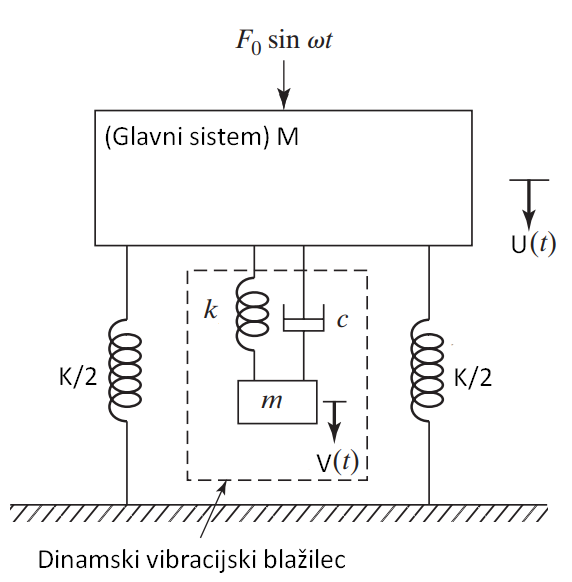
\includegraphics[scale=0.65]{slike/teorija/sistem_2ps.png}
            \caption{Nedušen sistem z DVB-jem}\label{fig:sistem_2ps}
        \end{figure}
        
        \newpage
        Izhodišče obravnave sta gibalni enačbi sistema za maso $M$ in $m$, pri čemer na prvo maso vpliva harmonično delujoča obremenitev z amplitudo $F_0$ in krožno frekvenco $\omega$:
        \begin{align}
            M \ddot U +K u + c (\dot U - \dot V) + k (U-V)  &= F_0 \sin\omega t \nonumber \,, \\
            m \ddot V + c (\dot V - \dot U) + k(V-U) &= 0 \, .
        \end{align}
        Predpostavimo harmonski odziv:
        \begin{align}
            U  &= U_0 \sin\omega t \nonumber \,,\\
            V  &= V_0 \sin\omega t
        \end{align}
        in za sistem enačb izpeljemo izraze amplitud mas $m$ in $M$:
        \begin{align}
            U_0&=\frac{F_0\left(k-m \, \omega^2+i \, c \, \omega\right)}{\left[\left(K-M \omega^2\right)\left(k-m \, \omega^2\right)-m \, k \, \omega^2\right]+i \, \omega \, c\left(K-M \omega^2-m \, \omega^2\right)}  \label{eq:X1_amplituda} \,,\\
            V_0&=\frac{U_0\left(k+i \, \omega \, c\right)}{\left(k-m \, \omega^2+ i \, \omega \, c\right)} \label{eq:X2_amplituda} \,.
        \end{align}
        
        Bistvo problema je zmanjšanje amplitude $U_0$, ki predstavlja velikost odziva glavnega sistema. Definiramo razmerje mas $\beta=m/M$, razmerje naravnih frekvenc glavnega sistema $\omega_0^2=K/M$, razmerje naravnih frekvenc resonatorja $\kappa_0^2=k/m$, razmerje naravnih frekvenc $\varkappa=\omega_0 / \kappa_0$, razmerje vzbujevalne frekvence in lastne frekvence glavnega sistema $\Omega=\omega/\omega_0$ in razmernik dušenja $\zeta=c/(2m\omega_0)$. Amplitude $U_0$ in $V_0$, lahko izrazimo s spodnjimi enačbami in za $m/M=1/20$ in nekaj različnih vrednosti $\zeta$ prikažemo odziv glavnega sistema z DVB-jem na sliki \ref{fig:sistem_2ps_2}. Torej:
        \begin{align}
            \frac{U_0}{F_0/K}=\left[\frac{(2 \zeta \Omega)^2+\left(\Omega^2-\varkappa^2\right)^2}{(2 \zeta \Omega)^2\left(\Omega^2-1+\beta \Omega^2\right)^2+\left\{\beta \varkappa^2 \Omega^2-\left(\Omega^2-1\right)\left(\Omega^2-\varkappa^2\right)\right\}^2}\right]^{1 / 2}\,,\\
            \frac{V_0}{F_0/K}=\left[\frac{(2 \zeta \Omega)^2+\varkappa^4}{(2 \zeta \Omega)^2\left(\Omega^2-1+\beta \Omega^2\right)^2+\left\{\beta \varkappa^2 \Omega^2-\left(\Omega^2-1\right)\left(\Omega^2-\varkappa^2\right)\right\}^2}\right]^{1 / 2}\,.
        \end{align}
        \begin{figure}[!hb]
            \centering
            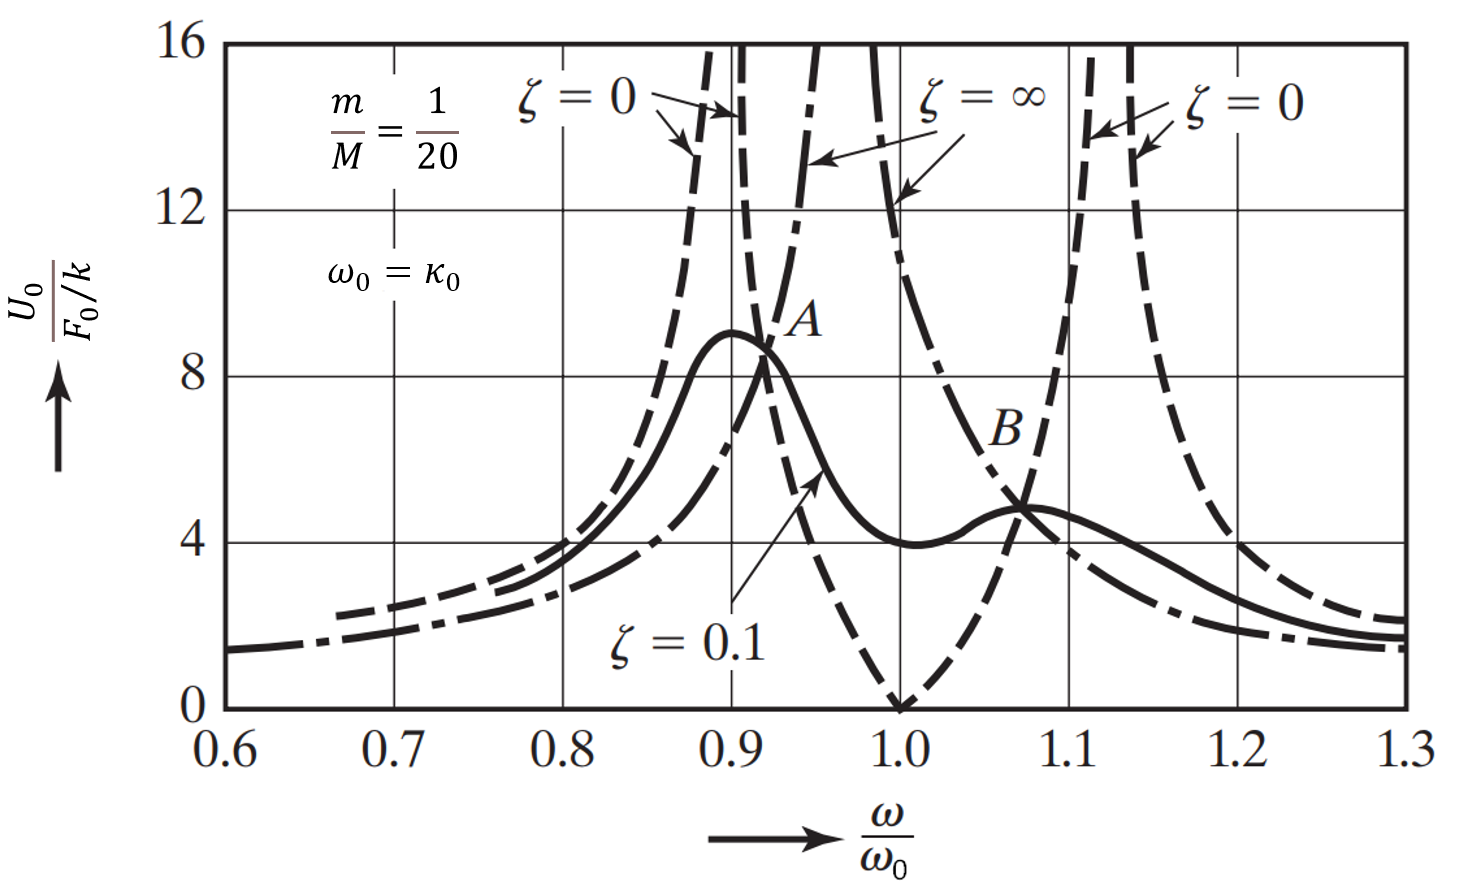
\includegraphics[scale=0.34]{slike/teorija/ozadje_problema.png}
            \caption{Dušen sistem z DVB-jem.}\label{fig:sistem_2ps_2}
        \end{figure}

        Za primer dušenja $c=\zeta=0$ lahko vidimo, da je:
        \begin{align}
            (k-m \, \omega^2) F_0 &= 0 \nonumber \,,\\
            \omega^2&=\frac{k}{m}\,.
        \end{align}
        Če smo torej prvotni sistem vzbujali z krožno frekvenco blizu prve krožne frekvence: 
        \begin{align}
            \omega^2 \simeq \omega_0^2=\frac{K}{M} ,
        \end{align}
        sledi iz zgornjih enačb pogoj za dimenzioniranje DVB-ja pri zanemarljivem dušenju:
        \begin{align}\label{eq:enakost_frekvenc}
            \omega^2 =\frac{K}{M} =\frac{k}{m} \,,
        \end{align}
        pri čemer je amplituda odziva z dodanim DVB-jem, kjer še vedno obratujemo pri originalnih pogojih z frekvenco $\omega_0$, tako nič. Z drugimi besedami je ustrezno dimenzioniran DVB tak, ki ima razmerje med svojo togostjo in maso enako kot je razmerje med togostjo in maso glavnega sistema. 
        
        Iz slike \ref{fig:sistem_2ps_2} je razvidno, da v točki A in B vse krivulje sovpadajo neodvisno od dušenja. Z prisotnostjo dušenja pogoj \eqref{eq:enakost_frekvenc} postane:
        \begin{align}
            \Omega=\frac{1}{1+\beta}\,,
        \end{align}
        dobimo še dodatni pogoj za najboljše razmerje dušenja:
        \begin{align}
            \zeta_{opt}^2=\frac{3\beta}{8(1+\beta)^3}\,.
        \end{align}

        V tem poglavju smo torej ugotovili, da lahko zmanjšamo odziv glavnega sistema z ustreznim dimenzioniranjem dinamičnega vibracijskega blažilca. Vidimo tudi, da ima DVB veliko pomanjkljivost. Majhen odziv sistema povzroči le v ozkem območju okoli prvotne lastne frekvence $\omega_0$. 
        
        V primeru, da se vzbujevalna frekvenca ali lastnosti sistema glede na prvotno dimenzioniranje spremenijo, DVB ne bo več tako učinkovit, v okolici izven območja dušenja lahko pride celo do povečanja amplitud. Z ustreznim krmiljenjem mase $m$ ali togosti $k$ lahko povečamo uporabno območje DVB-ja. V našem primeru, kjer segrevamo GPLA in tako vplivamo na modul elastičnosti, lahko spreminjamo togost resonatorja ROC-ja. 
        
        Velja tudi, da je lastne frekvenca $\omega_0=\sqrt{k/m}$ odvisna od togosti $k$. za dušenje nizkih frekvenc bi potrebovali zelo majhno togost $k$, ki jo pri MM uresničimo z nelinearnostjo. 
        
        V sledečem poglavju \ref{sec:metamaterial_dinamika} apliciramo teorijo 1D DVB na prej dimenzionirani ROC in tvorimo metamaterialno verigo z lastnostjo PZF. 
    
    \newpage
    \section{Dinamika neskončne periodične verige}\label{sec:metamaterial_dinamika}
        
        Enodimenzionalni kvazi-ničelni togostni metamaterial (1D KNT MM) lahko predstavimo kot model verige $j$-tih mas-togosti-dušilcev, ki je prikazan na sliki \ref{fig:MM_veriga}. V MM verigi, se v okvirju mase $M$ nahaja resonator mase $m$. Vsak okvir ima prostostno stopnjo $U_j$ in vsak resonator $V_j$. Resonatorji so v okvirje vpeti preko vzmeti z nelinearno karakteristično togostjo $k=k_{\mathrm{ROC}}$, ki v ROC povzroča silo $F_{\mathrm{ROC}}$ in ima koeficient dušenja $c$. Posamezne osnovne celice so med seboj povezane v verigo preko vzmeti, ki jo tvorita dva elementa pozitivne togosti $K=2 k_p$ (\cite{cai2020design}, \cite{lazarov2007low} ). 
        \begin{figure}[!hb]
            \centering
            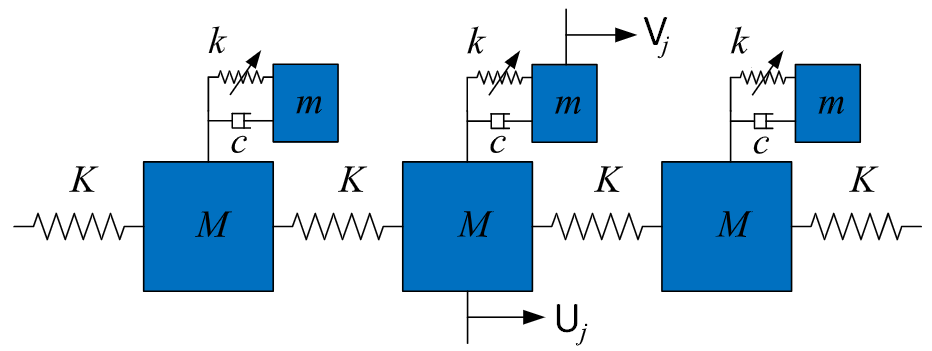
\includegraphics[scale=0.42]{slike/teorija/MM_veriga.png}
            \caption{enodimenzionalna metamaterialna veriga.}\label{fig:MM_veriga}
        \end{figure}
        
        Ko je število ROC neskončno, ali zadosti veliko, se tvori periodičnost verige, kjer ima vsaka celica periodične robne pogoje. Z $j$-to ROC lahko zapišemo gibalne enačbe: 
        \begin{align}
            M \ddot{U}_j+2 K U_j-K U_{j-1}-K U_{j+1}+c\left(\dot{U}_j-\dot{V}_j\right)+F_{\mathrm{ROC}}(U_j-V_j)&=0 \label{eq:gib_en_ROC_1} \\
            m \ddot{V}_j+c\left(\dot{V}_j-\dot{U}_j\right)+F_{\mathrm{ROC}}\left(V_j-U_j\right)&=0 \label{eq:gib_en_ROC_2} \,.
        \end{align}
        Za analizo pretvorimo enačbi v brezdimenzijsko obliko z vpeljavo: 
        \begin{align}
            &\tau=\omega_0 t, \quad  u_j=\frac{U_j}{L_0}, \quad v_j=\frac{V_j}{L_0}, \quad q_j=v_j-u_j, \quad \zeta=\frac{c}{2\sqrt{k \, m}} \nonumber \\ 
            &\alpha=\frac{k}{K}, \quad \beta=\frac{m}{M}, \quad \omega_0=\sqrt{\frac{K}{M}}, \quad \kappa_0=\sqrt{\frac{k}{m}}, \quad \varkappa=\sqrt{\frac{\kappa_0}{\omega_0}}=\sqrt{\frac{\alpha}{\beta}}\,.
        \end{align}
        Razen $\tau$, ki predstavlja brezdimenzijski čas, smo spremenljivke že definirali v poglavju \ref{sec:dvomasni_dušilec_nihanj}. Vpeljemo tudi brezdimenzijsko silo $f_{\mathrm{ROC}}=F_{\mathrm{ROC}}/(k_v L_0)$ iz dela \ref{sec:staticna_analiza_ROC}. Nadaljnji časovni odvodi diferencialnih enačb \eqref{eq:gib_en_ROC_1} in \eqref{eq:gib_en_ROC_2} so tako po brezdimenzijskem času:
        \begin{align}
            u_{j}''+2 u_{j} - u_{j-1} - u_{j+1} - 2 \zeta \beta \varkappa q_{j}' - \alpha f_{\mathrm{ROC}}(q_{j}) &= 0  \label{eq:gib_en_ROC_3} \,,\\
            q_{j}''+2 \zeta \varkappa q_{j}'+ \varkappa^2 f_{\mathrm{ROC}} (q_{j}) + u_{j}''&=0  \label{eq:gib_en_ROC_4} \,.
        \end{align}
        Za nadaljnjo analizo brezdimenzijsko silo $f_{\mathrm{ROC}}(q_j)$ v enačbi \eqref{eq:brezdimenzijski_f(x)} v okolici ravnovesne lege $q_j=0$ s pomočjo Taylorjeve aproksimacije razvijemo v:
        \begin{align}
            f_{\mathrm{ROC}}(q_j) = \frac{1}{2}\left(2+\mu-\frac{\mu}{\gamma}\right)  q_j + \frac{\mu }{4 \gamma^3} q_j^3 -\frac{3 \mu }{16 \gamma^5} q_j^5 + \frac{5 \mu}{32 \gamma^7} q_j^7 + ...
        \end{align}
        Z upoštevanjem enačb \eqref{eq:KNT_pogoj_1}, \eqref{eq:KNT_pogoj_2} ter aproksimacije petega reda dobimo:
        \begin{align}
            f_{\mathrm{ROC}}(q_j) \approx \frac{1}{2 \gamma^2(1-\gamma)} q_j^3-\frac{3}{8  \gamma^4 (1-\gamma)} q_j^5 \nonumber \,, \\
            f_{\mathrm{ROC}}(q_j) \approx \delta q_j^3 + \eta q_j^5\,.
        \end{align}
        
        Analitična rešitev nelinearnega sistema enačb \eqref{eq:gib_en_ROC_3} in \eqref{eq:gib_en_ROC_4} ni znana. Aproksimativno rešitev je mogoče dobiti z uporabo metode harmonskega ravnotežja \cite{huang2016harmonic}, \cite{thomsen2003vibrations}. Predpostavimo periodični odziv pomika $q_j(\tau)$ v obliki kompleksne Fouriereve vrste: 
        \begin{equation}
        \begin{aligned}
            q_{k, j}(\tau) &=\sum_k \epsilon^{(k-1) / 2} A_{k, j} \mathrm{e}^{\mathrm{i} k \Omega \tau}+\epsilon^{(k-1) / 2} \overline{A}_{k, j} \mathrm{e}^{-\mathrm{i} k \Omega \tau}, \quad k &=1, 3, 5, \ldots \,, 
        \end{aligned}
        \end{equation}
        
        kjer je $\epsilon$ brezdimenzijski parameter, ki kaže na red amplitude gibanja in $\Omega=\omega/\omega_0$ normirana lastna krožna frekvenca. Višje rede zanemarimo in za $k=1$ dobimo:
        \begin{equation}\label{eq:nastavek_qj}
            q_j(\tau)=A_j \mathrm{e}^{i\Omega \tau}+\overline{A}_j \mathrm{e}^{-i\Omega \tau} \,.
        \end{equation}
        
        Nastavek vstavimo v enačbo \eqref{eq:gib_en_ROC_4} in dvojno integriramo glede na $\tau$, kjer dobimo izraz odziva $j$-te mase, ter pri tem zanemarimo člene višjega reda $\mathcal{O}(A_j \mathrm{e}^{3 i \Omega \tau})$:
        \begin{align}\label{eq:nastavek_uj}
            u_j=&\frac{A}{\Omega^2}\left[ A_j \overline{A}_j (3\delta+10 A_j \overline{A}_j \eta)\varkappa^2 + 2 i \zeta \varkappa \Omega-\Omega^2 \right]  \mathrm{e}^{i \Omega \tau} + ...\nonumber\\
            & ... + \frac{B}{\Omega^2}\left[ A_j \overline{A}_j (3\delta+10 A_j \overline{A}_j \eta)\varkappa^2 + 2 i \zeta \varkappa \Omega-\Omega^2 \right] \mathrm{e}^{-i \Omega \tau}  + \mathcal{O}(A_j \mathrm{e}^{3 i \Omega \tau}) \,.
        \end{align}
        
        Nastavek \eqref{eq:nastavek_qj} in zgornjo enačbo \eqref{eq:nastavek_uj} vstavimo v \eqref{eq:gib_en_ROC_3} in nastavimo koeficiente pred $\mathrm{e}^{	\pm i \Omega \tau}$ na nič. Dobimo amplitudno-frekvenčni enačbi:
        \begin{align}
            A_{j-1}+A_{j+1}-&A_{j}\left(2+ A_{j} \overline{A}_{j}(3 \delta+10 A_{j} \overline{A}_{j} \eta)\left(\alpha+\varkappa ^2\right)\right) - ...\nonumber \\
            ... &-\frac{3\delta\varkappa^2}{\Omega^2}\left(A_{j-1}^2 \overline{A}_{j-1}-2 A_{j}^2 \overline{A}_{j}+A_{j+1}^2 \overline{A}_{j+1}\right) - ... \nonumber \\
            ... & - \frac{10\eta\varkappa^2}{\Omega^2}\left(A_{j-1}^3 \overline{A}_{j-1}^2-2 A_{j}^3 \overline{A}_{j}^2+A_{j+1}^3 \overline{A}_{j+1}^2\right) -     ... \nonumber\\
            ... &- \frac{2 i(A_{j-1}-2 A_{j}+A_{j+1}) \zeta \varkappa }{\Omega} -2 i A_{j}  (1+\beta) \zeta \varkappa  \Omega+A_{j} \Omega^2 = 0 \,,
        \end{align}
        \begin{align}
            \overline{A}_{j-1}+\overline{A}_{j+1}-&\overline{A}_{j}\left(2+A_{j} \overline{A}_{j}(3 \delta+10 A_{j} \overline{A}_{j} \eta)\left(\alpha+\varkappa ^2\right)\right) - ...\nonumber \\
            ... &-\frac{3\delta\varkappa^2}{\Omega^2}\left(A_{j-1} \overline{A}_{j-1}^2-2 A_{j} \overline{A}_{j}^2+A_{j+1} \overline{A}_{j+1}^2\right) - ... \nonumber \\
            ... & - \frac{10\eta\varkappa^2}{\Omega^2}\left(A_{j-1}^2 \overline{A}_{j-1}^3-2 A_{j}^2 \overline{A}_{j}^3+A_{j+1}^2 \overline{A}_{j+1}^3\right) -     ... \nonumber\\
            ... &- \frac{2 i(A_{j-1}-2 A_{j}+A_{j+1}) \zeta \varkappa }{\Omega} -2 i A_{j} (1+\beta) \zeta \varkappa  \Omega+A_{j} \Omega^2 = 0 \,.
        \end{align}
        
        V zgornje enačbe lahko vstavimo specifične vrednosti amplitud mase $j$ kot tudi sosednjih mas $j+1$ in $j-1$, dobimo sistem enačb za amplitudo odziva pritrjenega oscilatorja. Sistem je nelinearen in ima posledično lahko več rešitev. Amplitudo vala, ki potuje po MM verigi dobimo tako, da vstavimo amplitudo pritrjenega oscilatorja v enačbo \eqref{eq:nastavek_uj}.
        
        \newpage
        Val, ki potuje po MM verigi preko pomikov $u_j$ lahko določimo tudi tako, da definiramo faktor širjenja valovanja $\mu_u$, ki predstavlja valovno število $k_u$ pomnoženo z razdaljo med masami ROC-jev $L_u$. Pomika sosednjih mas, lahko definiramo kot:
        \begin{equation}
            u_{j \pm 1}= B_j \mathrm{e}^{\pm i \mu_u} \mathrm{e}^{\mathrm{i} \Omega \tau} + 
            \overline{B_j} \mathrm{e}^{\pm i \mu_u} \mathrm{e}^{-\mathrm{i} \Omega \tau}\,,
        \end{equation}
        
        pri čemer so $B_j$ in $\overline{B}_j$ koeficienti pred $\mathrm{e}^{\pm i\Omega \tau}$ enačbe \eqref{eq:nastavek_uj}. Zgornjo enačbo, kot tudi enačbo \eqref{eq:nastavek_qj} vstavimo v enačbo \eqref{eq:gib_en_ROC_3}, enačimo koeficiente pred $ \mathrm{e}^{\pm i\Omega \tau}$ z nič in rešimo za $\mu_u$, ter tako dobimo enačbo disperzijskih krivulj:
        \begin{align}\label{eq:disperzijska_krivulja}
            \cos{\mu_u}=1-\frac{\Omega}{2}
            -\frac{\Omega^2}{2} \left[ \frac{\alpha(3 \delta A_j \overline{A}_{j}  + 10 \eta A_j^2 \overline{A}_{j}^2  ) + 2 i \beta \zeta \varkappa \Omega}{\varkappa^2 (3 \delta A_j \overline{A}_{j}  + 10 \eta  A_j^2 \overline{A}_{j}^2 ) - \Omega^2 + 2 i \zeta \varkappa \Omega} \right] \,.
        \end{align}
        
        Disperzijske krivulje so grafično prikazane na sliki (\ref{fig:teoreticna_disperzijska}), kjer so prikazane realne in imaginarne komponente rešitve. Končno lahko zapišemo razmerje med $M_j$-to in $M_{j+1}$-to maso kot:
        \begin{equation}
            u_{j+1}=\mathrm{e}^{\Im{\mu}} u_j \, \mathrm{e}^{-i \Re{\mu}} \,.
        \end{equation}
        
        Do dušenja mehanskih valov v verigi pride v tako imenovani pasovni vrzeli, kjer je $\mathrm{e}^{\Im{\mu}}$ manj kot $1$. Valovi pri drugih frekvencah izven pasovne vrzeli, potujejo brez izgube energije. Dodatno velja, da je fazni zamik $\Re{\mu}$ potujočega vala odvisen od $\mu$. Znotraj pasovne vrzeli, je dušenje največje pri minimumu $\mathrm{e}^{\Im{\mu}}$, torej pri $\Omega=\varkappa$. Z drugimi besedami, je frekvenca vzbujanja enaka lastni frekvenci resonatorjev $\Omega=\kappa_0$.
        \begin{figure}[!hb]
            \centering
            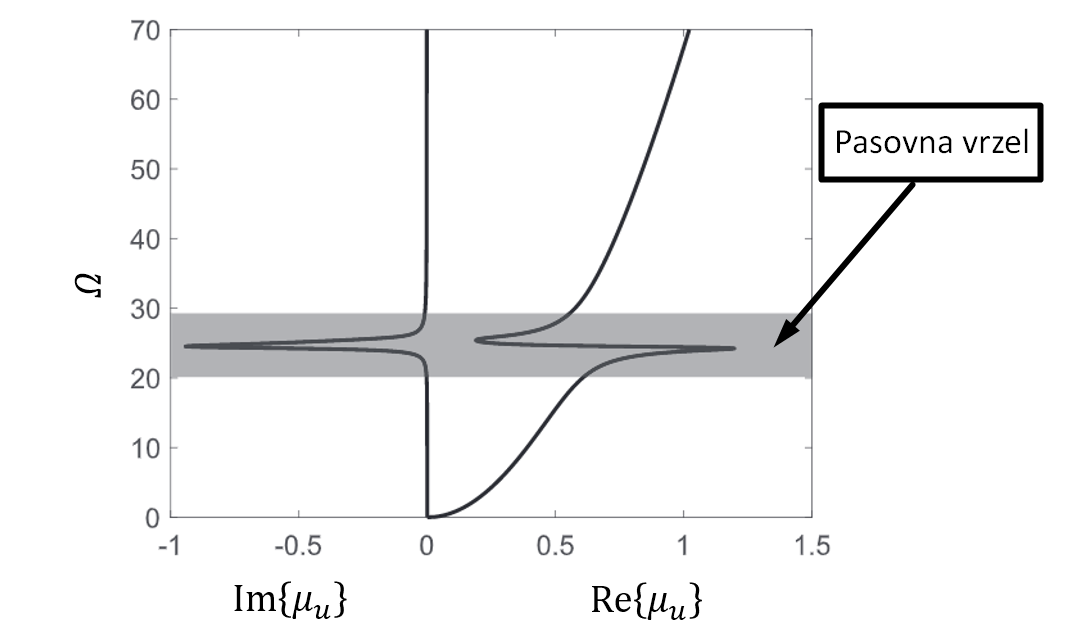
\includegraphics[scale=0.50]{slike/teorija/disperzijska_teorija.png}
            \caption{enodimenzionalna metamaterialna veriga.}\label{fig:teoreticna_disperzijska}
        \end{figure}
        
        
        